\header{
    \headtitle{Marée basse} \label{maree-basse}
    %
    
    \insertComment{Chanson des Amis d'ta femme (2000).}{}
}

\enluminure{4}{\href{https://www.youtube.com/watch?v=M1avvoQ1o4g}{J}}{e ne sais} pas pour vous
\\Mais pour ce qui est de moi,
\\Faudrait que j'boive un coup,
\\Tout, n'importe quoi,
\\Ca fera bien l'affaire,
\\A force de chanter,
\\De hurler et de braire,
\\J'ai besoin d'picoler.
\\Mais qu'on ne me serve pas
\\Du jus d' fruit ou de la flotte.
\\Surtout pas d'coca :
\\Je tiens trop à ma glotte
\dualcol{
\textbf{Refrain :}
\\Patron ! y'a marée basse !
\\Fais moi voir la p'tite soeur !
\\J'ai le gosier qui s'lasse
\\D'êt' tout sec. Quelle horreur !!
\\\\Un bon demi bien frais,
\\Pour y mettre du goût,
\\Le Picon y a qu'ça d'vrai !
\\Ou même un petit rouge.
\\Un bon vieux jaja,
\\Plus ça tâche et mieux c'est.
\\Ou bien un pastaga.
\\Mais sans glaçons s'te plait.
\\Tequila, gin, vodka,
\\Rhum ou encore whisky
\\Sers moi tout c'que tu as,
\\Tu me sauves la vie !
\\\\J'ai besoin d'fortifiant
\\Y en a bien des qui s'dopent
\\L'alcool c'est important
\\Pour qu'l'humeur se développe.
\\Et même si ça rend beauf'
\\Quoi qu'ça dépend pour qui :
\\L'hiver ça me réchauffe,
\\L'été ça m'rafraîchit !
\\Et tant pis pour mon foie,
\\On crèv'ra tous, ça se fête.
\\Autant vivre dans la joie.
\\Merde on n'est pas des bêtes !!!!
\begin{center}
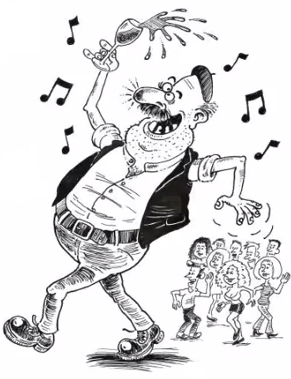
\includegraphics[width=0.4\textwidth]{images/maree_basse.png}
\end{center}
}

\breakpage